\section{MLOps}\label{sec:mlops}

In this section we will try to describe key aspect of MLOps as can be found in today's literature.

\subsection{Description}\label{subsec:description}
MLOps or Machine Learning Operations is the automation of Machine learning development workflow and operations.
It's an extension of DevOps practices adapted to machine learning model development and data operations.
MLOps almost never taken alone and DataOps is an integrated part of the full MLOps lifecycle (articles,).

MLOps with clearly defined workflow and infrastructure can provide transparency and accountability to Upper Management and Business.\cite{treveil2020introducing}(p.11)
You don't need to be an engineer to understand the flow of operations and what is required to work it out.

\begin{figure}[!htbp]
    \caption{MLOps lifecycle\cite{mlops-definition-tools-and-challenge}}
    \centering
    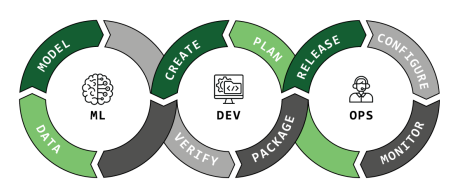
\includegraphics[scale=0.5]{images/ml-dev-ops}
    \label{fig:ml-dev-ops}
\end{figure}

MLOps is essential for data teams and organizations, as it involves a complex integration of technologies, processes, and people, requiring ongoing discipline and time to implement effectively.
It is not a one-time task but a continuous effort to ensure successful machine learning operations.\cite{treveil2020introducing}(p.38)


\subsection{Why MLOps?}

A survey in 2021\cite{DBLP:journals/corr/abs-2103-08942} already show that Machine Learning development is evolving towards team-based development.
They also show that in a result the adoption of DevOps practices is increasing and the required skills in infrastructure and deployment are evolving.

In this regard, they also identified the following obstacles among others\cite{DBLP:journals/corr/abs-2103-08942}:
    \begin{itemize}
        \item Accessibility of data
        \item Building training pipelines
        \item Deployment and target environment (on-premise, cloud)
        \item Tracking and comparing training
        \item Collaborating on projects
        \item Lack of guidelines
    \end{itemize}

Since then, we will see that some of those difficulties have been tackled, tools exist and are currently reviewed in the literature.

\subsection{Roles in MLOps}\label{subsec:actors}

\begin{figure}[!htbp]
    \caption{Realistic picture of a machine learning model life cycle inside an average
    organization today\cite{treveil2020introducing}(p.6)}
    \centering
    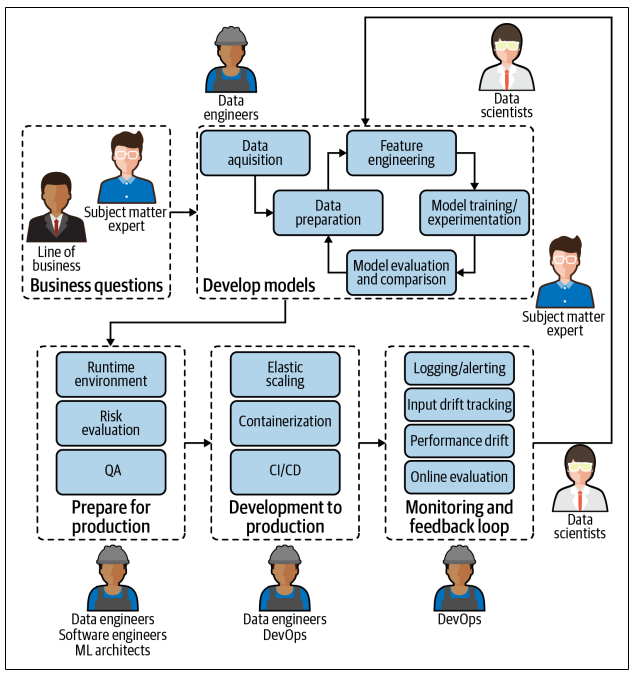
\includegraphics[scale=0.5]{images/mlops-people}
    \label{fig:mlop-people}
\end{figure}

As we already said, Machine learning development is now team based and requires collaboration across diverse roles.
From business experts to technical architects each role contributes to the lifecycle of machine learning models.
They will ensure maintenance, optimization, build and deployment trust, and mitigate business risks\cite{treveil2020introducing}(p.22).

Data scientist is the obvious starting role.
Around the data scientist, in the context of MLops the literature
propose roles\cite{treveil2020introducing}(p.14),
\begin{itemize}
    \item Subject-Matter Experts
    \item Data Scientists
    \item Data Engineers
    \item DevOps engineers
    \item Software engineers
    \item Model Risk Managers
    \item Machine Learning architects
\end{itemize}

\textit{Each person—from the subject-matter-expert on the business side to the most
technical machine learning architect—plays a critical part in the maintenance of ML
models in production}\cite{treveil2020introducing}(p.22).

In figure \ref{fig:mlop-people}, they propose an example of those roles within an organization.




\subsection{Workflow}\label{subsec:workflow}


\subsubsection{Developing Models}

\begin{figure}[!htbp]
    \caption{Model development highlighted in the larger context of the ML project life
    cycle\cite{treveil2020introducing}(p.41)}
    \centering
    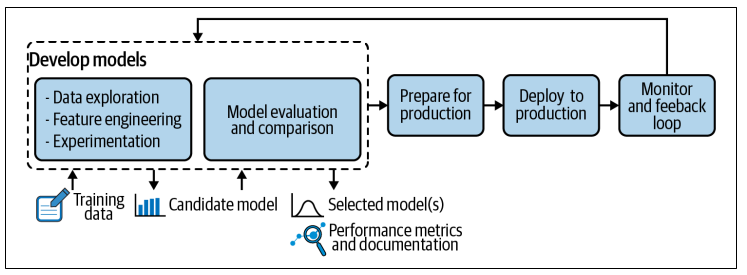
\includegraphics[scale=0.5]{images/developing-models-intro}
    \label{fig:developing-models-intro}
\end{figure}


\subsubsection{Prepare for production}

\begin{figure}[!htbp]
    \caption{Preparing for production highlighted in the larger context of the ML project
    life cycle\cite{treveil2020introducing}(p.59)}
    \centering
    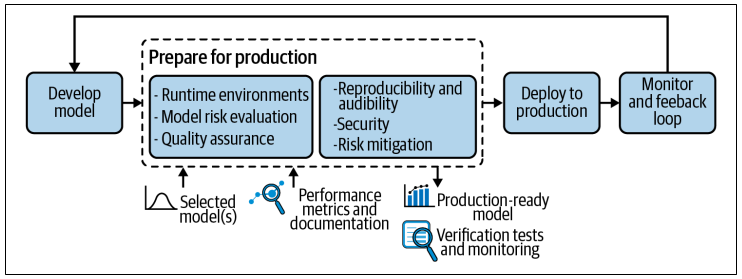
\includegraphics[scale=0.5]{images/prep-prod-intro}
    \label{fig:prep-prod-intro}
\end{figure}


\subsubsection{Deploy in production}

\begin{figure}[!htbp]
    \caption{Preparing for production highlighted in the larger context of the ML project
    life cycle\cite{treveil2020introducing}(p.73)}
    \centering
    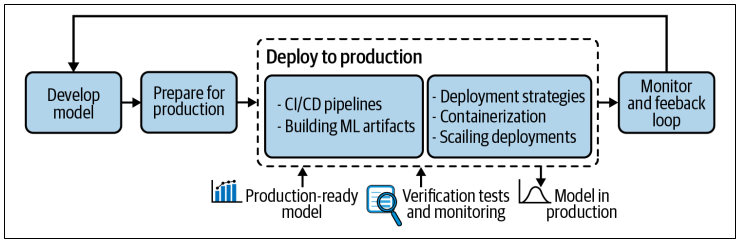
\includegraphics[scale=0.5]{images/deploy-prod}
    \label{fig:deploy-prod}
\end{figure}

CI/CD concepts apply to traditional software engineering, but they apply just as well
to machine learning systems and are a critical part of MLOps strategy. After success‐
fully developing a model, a data scientist should push the code, metadata, and docu‐
mentation to a central repository and trigger a CI/CD pipeline. An example of such
pipeline could be:
1. Build the model
a. Build the model artifacts
b. Send the artifacts to long-term storage
c. Run basic checks (smoke tests/sanity checks)
d. Generate fairness and explainability reports
2. Deploy to a test environment
a. Run tests to validate ML performance, computational performance
b. Validate manually
3. Deploy to production environment
a. Deploy the model as canary
b. Fully deploy the model
Many scenarios are possible and depend on the application, the risks from which the
system should be protected, and the way the organization chooses to operate. Gener‐
ally speaking, an incremental approach to building a CI/CD pipeline is preferred: a
simple or even naïve workflow on which a team can iterate is often much better than
starting with complex infrastructure from scratch.\cite{treveil2020introducing}(p.74)

\subsubsection{Monitor and FeedBack}

\begin{figure}[!htbp]
    \caption{Monitoring and feedback loop highlighted in the larger context of the ML
    project life cycle\cite{treveil2020introducing}(p.85)}
    \centering
    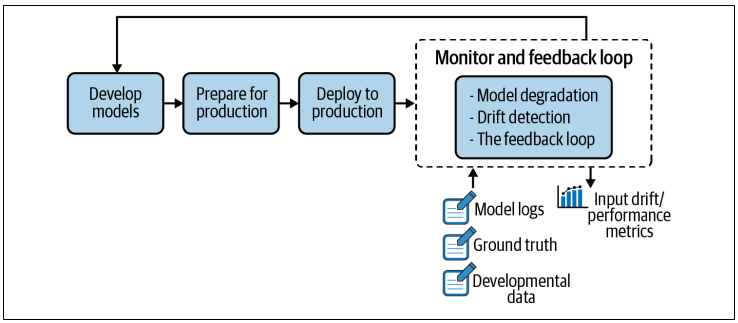
\includegraphics[scale=0.5]{images/monitor-intro}
    \label{fig:monitor-intro}
\end{figure}

How Often Should Models Be Retrained?
One of the key questions teams have regarding monitoring and retraining is: how
often should models be retrained? Unfortunately, there is no easy answer, as this
question depends on many factors, including:
The domain
Models in areas like cybersecurity or real-time trading need to be updated regu‐
larly to keep up with the constant changes inherent in these fields. Physical mod‐
els, like voice recognition, are generally more stable, because the patterns don’t
often abruptly change. However, even more stable physical models need to adapt
to change: what happens to a voice recognition model if the person has a cough
and the tone of their voice changes?
The cost
Organizations need to consider whether the cost of retraining is worth the
improvement in performance. For example, if it takes one week to run the whole
data pipeline and retrain the model, is it worth a 1\% improvement?
The model performance
In some situations, the model performance is restrained by the limited number of
training examples, and thus the decision to retrain hinges on collecting enough
new data.\cite{treveil2020introducing}(p.86)

Understanding Model Degradation
Once a machine learning model is trained and deployed in production, there are two
approaches to monitor its performance degradation: ground truth evaluation and
input drift detection. Understanding the theory behind and limitations of these
approaches is critical to determining the best strategy.\cite{treveil2020introducing}(p.89)

\begin{figure}[!htbp]
    \caption{Continuous delivery for end-to-end machine learning process\cite{treveil2020introducing}(p.95)}
    \centering
    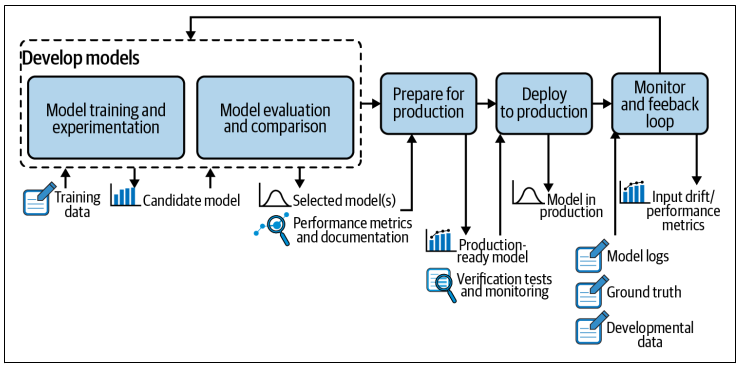
\includegraphics[scale=0.5]{images/feedback-loop-intro}
    \label{fig:feedback-loop-intro}
\end{figure}

Ordinary software is built to satisfy specifications. Once an application is deployed,
its ability to fulfill its objective does not degrade. ML models, by contrast, have objec‐
tives statistically defined by their performance on a given dataset. As a result, their
performance changes, usually for the worse, when the statistical properties of the data
change.
In addition to ordinary software maintenance needs (bug correction, release
upgrades, etc.), this performance drift has to be carefully monitored. We have seen
that performance monitoring based on the ground truth is the cornerstone, while
drift monitoring can provide early warning signals. Among possible drift mitigation
measures, the workhorse is definitely retraining on new data, while model modifica‐
tion remains an option. Once a new model is ready to be deployed, its improved per‐
formance can be validated thanks to shadow scoring or, as a second choice, A/B
testing. This enables proving that the new model is better in order to improve the
performance of the system.\cite{treveil2020introducing}(p.103)


\subsection{Maturity Models}\label{subsec:matutiry-models}
In\cite{mlops-maturity-model}, they propose a maturity model that goes from manual MLOps to fully automated MLOps.
It differs from the Microsoft and the Google MLOps maturity models,
but they all tend to go from manual to fully automated MLOps processes using automated CI/CD and
ML pipelines.\cite{mlops-definition-tools-and-challenge}

\begin{figure}[!htbp]
    \caption{Maturity levels \cite{mlops-maturity-model}}
    \centering
    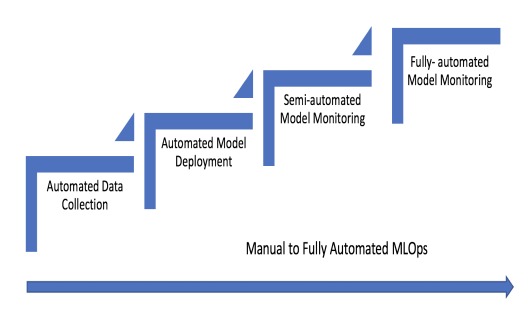
\includegraphics[scale=0.5]{images/maturity-levels}
    \label{fig:maturity}
\end{figure}


\subsection{MLOps is not AI for DevOps}\label{subsec:mlops-is-not-ai-for-devops}
In the literature, one might encounter the concept of Artificial Intelligence for DevOps (AI for DevOps)which is the study.
It's not the same as MLOps but of course as MLOps derives from DevOps it can also benefit from AI for DevOps,
but it's not the purpose of our actual research.